\subsection{Methodology}
\label{sec:dataset:architecture:methodology}

To understand the methodology on how we captured our dataset, we must first introduce the three key notions behind \gls{mde}: technical spaces, models and systems. A system is a concrete ``group or set of related or associated elements perceived or thought of as a unity or complex whole'' \citep{oed:system}. Technical spaces were introduced \citet{Bezivin:2002} as a model management framework based on algebraic structures (e.g., trees, (hyper)graphs, categories). Technical spaces are usually based on a three-tier conjecture: metametamodels, metamodels and models. Whereas a model is an abstract representation a concrete system of specific purpose, a \textit{meta}model, in contrast, describes the way to describe those models. A \textit{metameta}model can be used to describe the representation structure of our metamodels and defines a type system that supports all underlying layers \citep{Bezivin:2006gw}. Figure~\ref{fig:dataset:bezivin2006_metamodel} captures these concepts in further detail.

\begin{figure}[h]
  \centering
  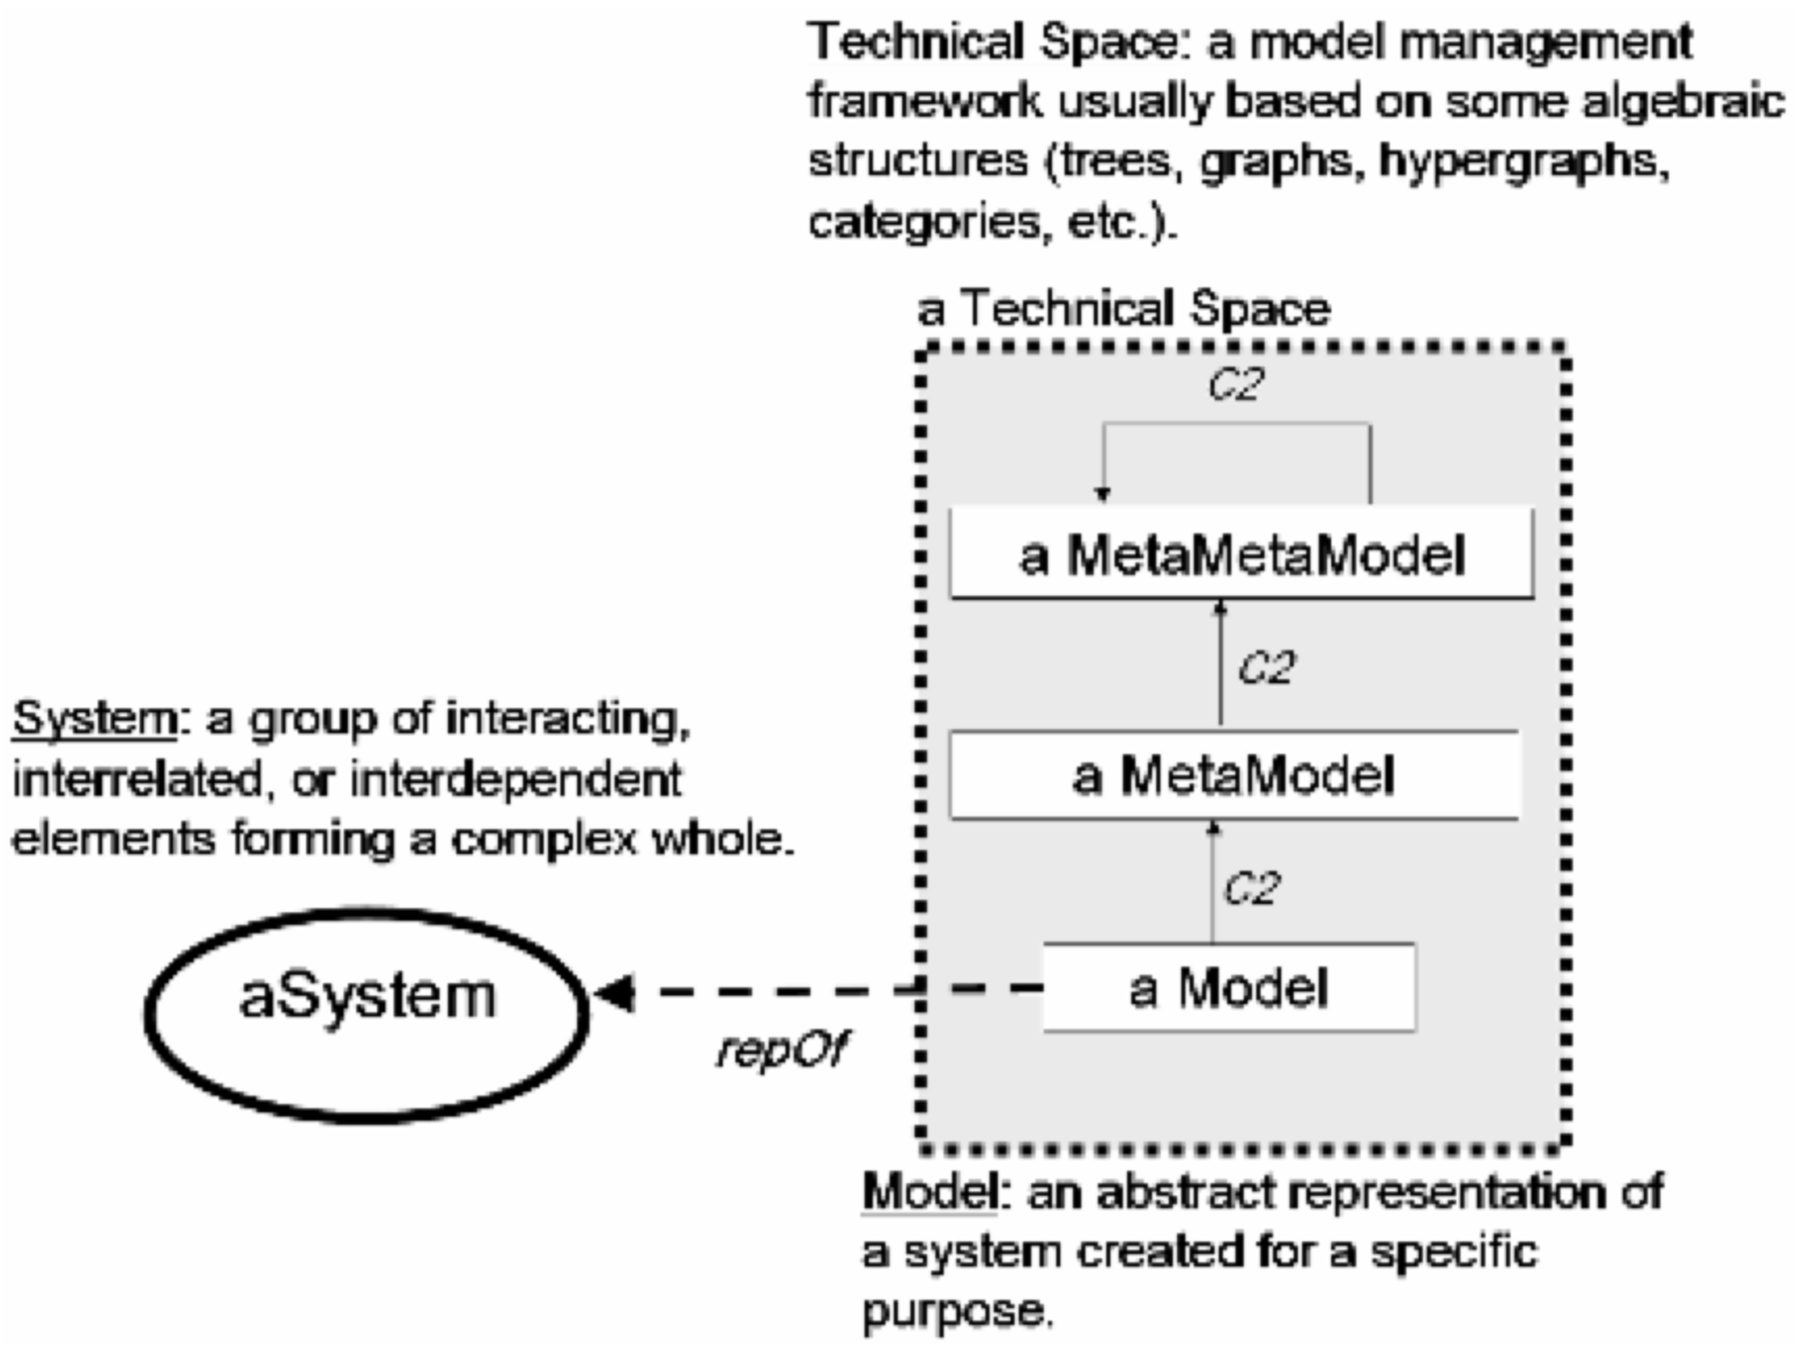
\includegraphics[width=0.6\textwidth]{images/dataset/bezivin2006_metamodel}
  \caption[An overview of systems, models and technical spaces]{Systems, models and technical spaces. (From \citep{Bezivin:2006gw}.)}
  \label{fig:dataset:bezivin2006_metamodel}
\end{figure}

We captured these concepts in a prototypical exploration process, first by developing a prototype system iteratively with a data tagging team who manually curated the data. Once this prototype was stable, we developed a model (Section~\ref{sec:dataset:architecture:what_to_capture}) around the prototype. We generalised the system we had developed, expanding from a model we had designed that was marathon-specific, into a more generalisable metamodel (Section~\ref{sec:dataset:architecture:metamodel}). We represent our process as as a \gls{uml} activity sequence diagram, shown in Figure~\ref{fig:dataset:methodology}.

The initial phase in our dataset development was to create a prototype system with the specific purpose of tagging our marathon runner context (using the dataset provided by the industry client). We name this partial implementation \textit{Argus}\footnoteurl{http://www.deakin.edu.au/~ca/argus}{5 July 2017}\footnote{Whose name is inspired by the \textit{all-seeing} giant of the same name from Greek mythology: ``With his multiple sets of eyes, Argus could see nearly everything in his vicinity''. See \url{http://www.loggia.com/myth/argus.html}.}. Refer to Section~\ref{sec:dataset:argus} for more about this implementation. 

To develop this initial model (and thus to then what our metamodel would be), we began by discussing what requirements were needed---that is, the key features that we thought were necessary for extracting from our image. Five features were decided: (1) the crowdedness of the photo, (2) the visible bib sheets within the photo, (3) the faces corresponding to those bib sheets, (4) the prominence of runners of the photo and (5) the colours of runners' clothing in the photo.

Once an initial prototype was developed, we conducted informal usability tests with members from \gls{dstil}, which captured minor flaws in the workflow (namely required conditions that were missing in annotations) as well as general usability enhancements. Once the internal testing had concluded, we developed instructional video guides on how to use Argus, and then deployed the tool to a data tagging team that made the data available to us.

After deployment, we ran four iterations of tagging with our external data tagging team. We use the term \textit{iteration} to refer to the process of deploying Argus to the data tagging team, capturing a set of photos from various races, and sending the data back for quality assurance. These iterations consisted of photos from different marathon races in our dataset. (To ensure variance in tagging, there were some races at night and some races with alphanumeric components in the \gls{rbn}.) After each iteration we assessed the tagging for quality. Feedback identified further restrictions that needed to be placed on Argus as poor approximations or incorrect tagging would cause our \gls{ai} to learn poorly. 

The following issues were identified:

\begin{itemize}
  \item face region was too far away from the bib region,
  \item face region was overlapping the bib region,
  \item \glspl{rbn} had spaces,
  \item misidentified \glspl{rbn} where the alphabetic `I' was tagged as the numeric `1'.
\end{itemize}

\noindent
Furthermore, we added geometric restrictions and conditions into the tool to prevent these errors from occurring at all (i.e., ensuring faces could only be marked above and horizontally near bibs). Some of these issues are highlighted in Figure~\ref{fig:dataset:issues_with_tagging}.

\begin{figure}[p]
  \centering
  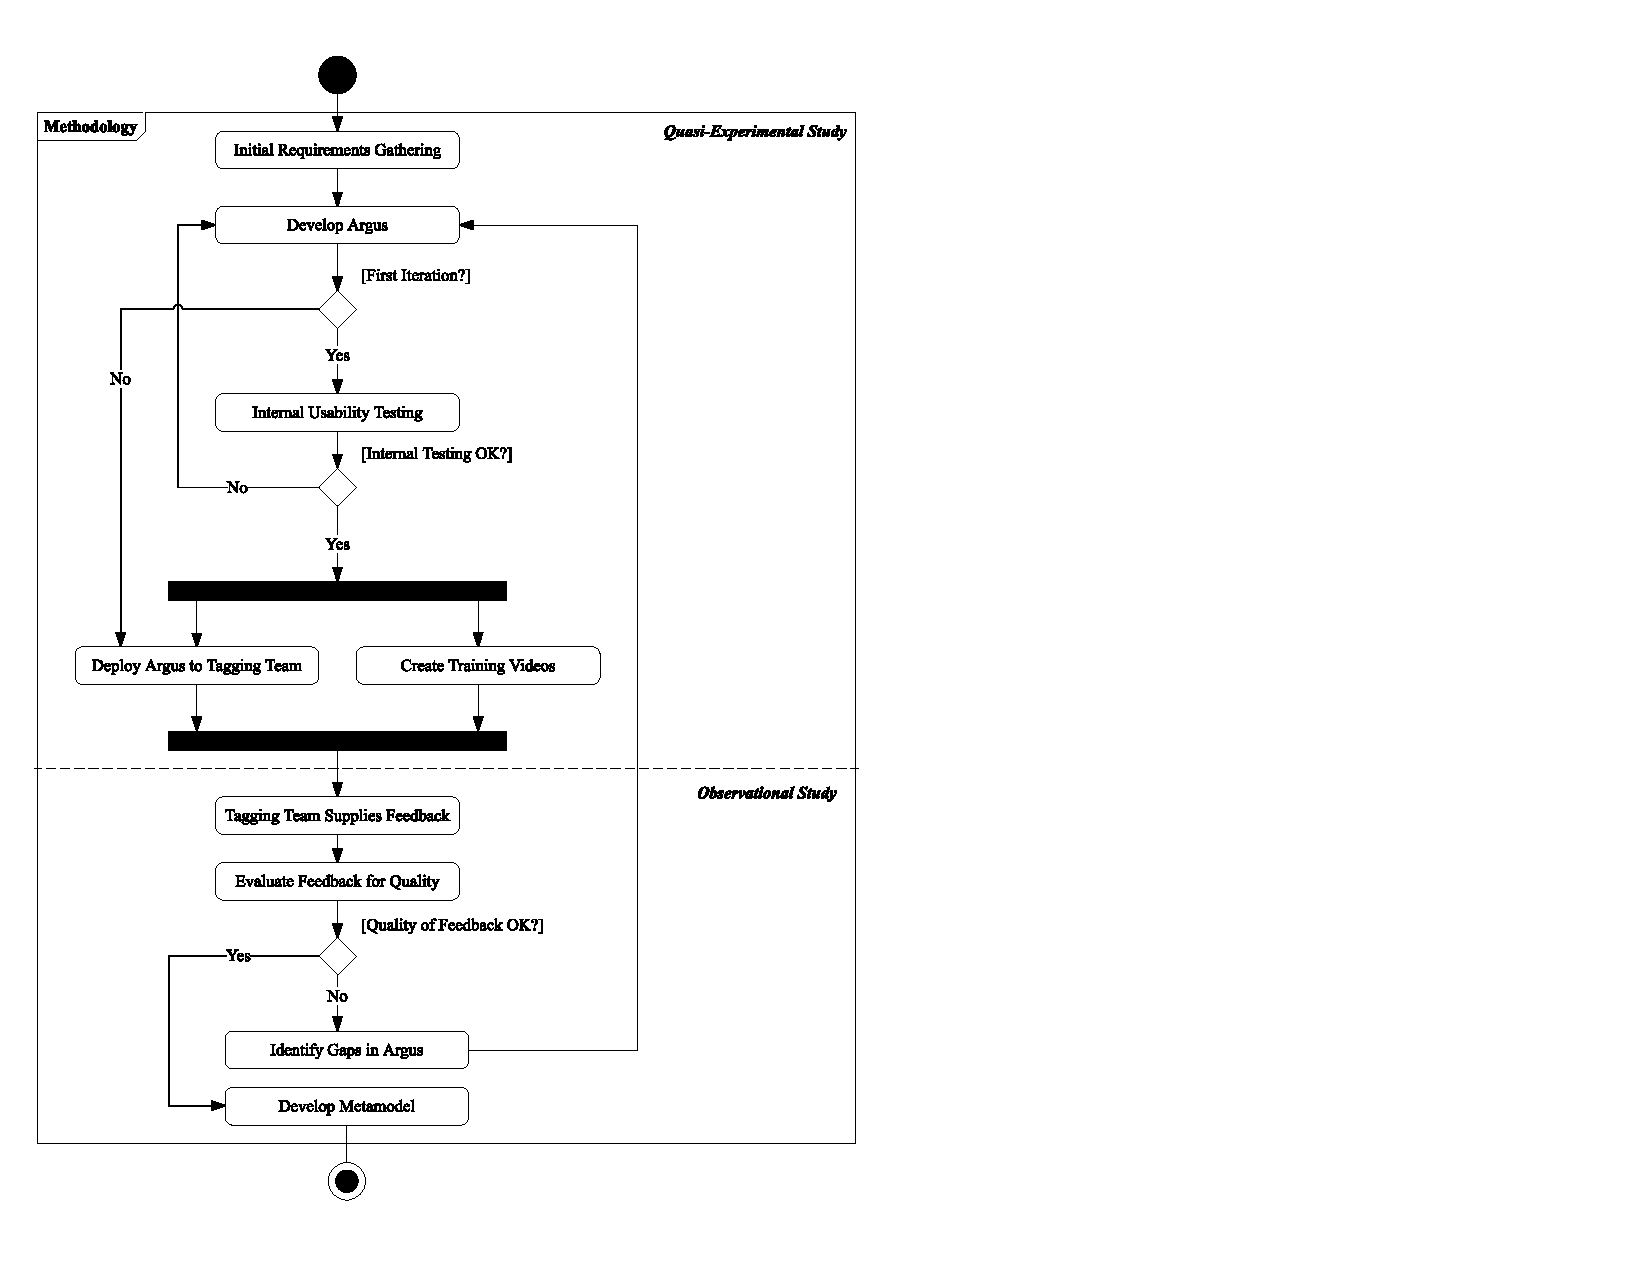
\includegraphics[width=0.7\textwidth]{images/dataset/methodology}
  \caption[Implementation methodology]{An overview of the methodology used to discover our metamodel.}
  \label{fig:dataset:methodology}
\end{figure}

\begin{figure}[p]
  \centering
  
  \begin{subfigure}[b]{0.8\textwidth}
    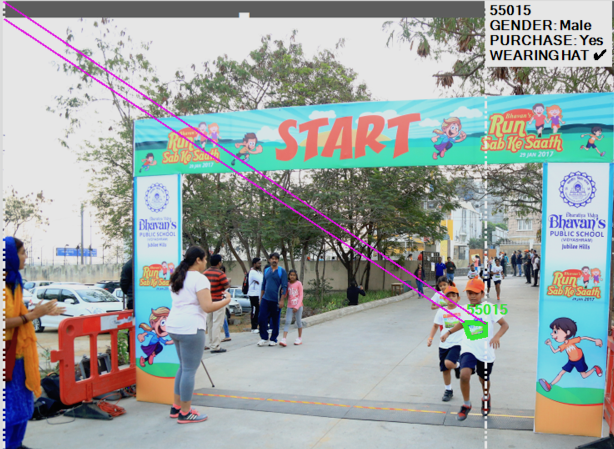
\includegraphics[width=\textwidth]{images/dataset/BadTagging_TooFar}
  \end{subfigure}\\
  \vspace{1cm}
  \hspace{\fill}
  \begin{subfigure}[b]{0.3\textwidth}
    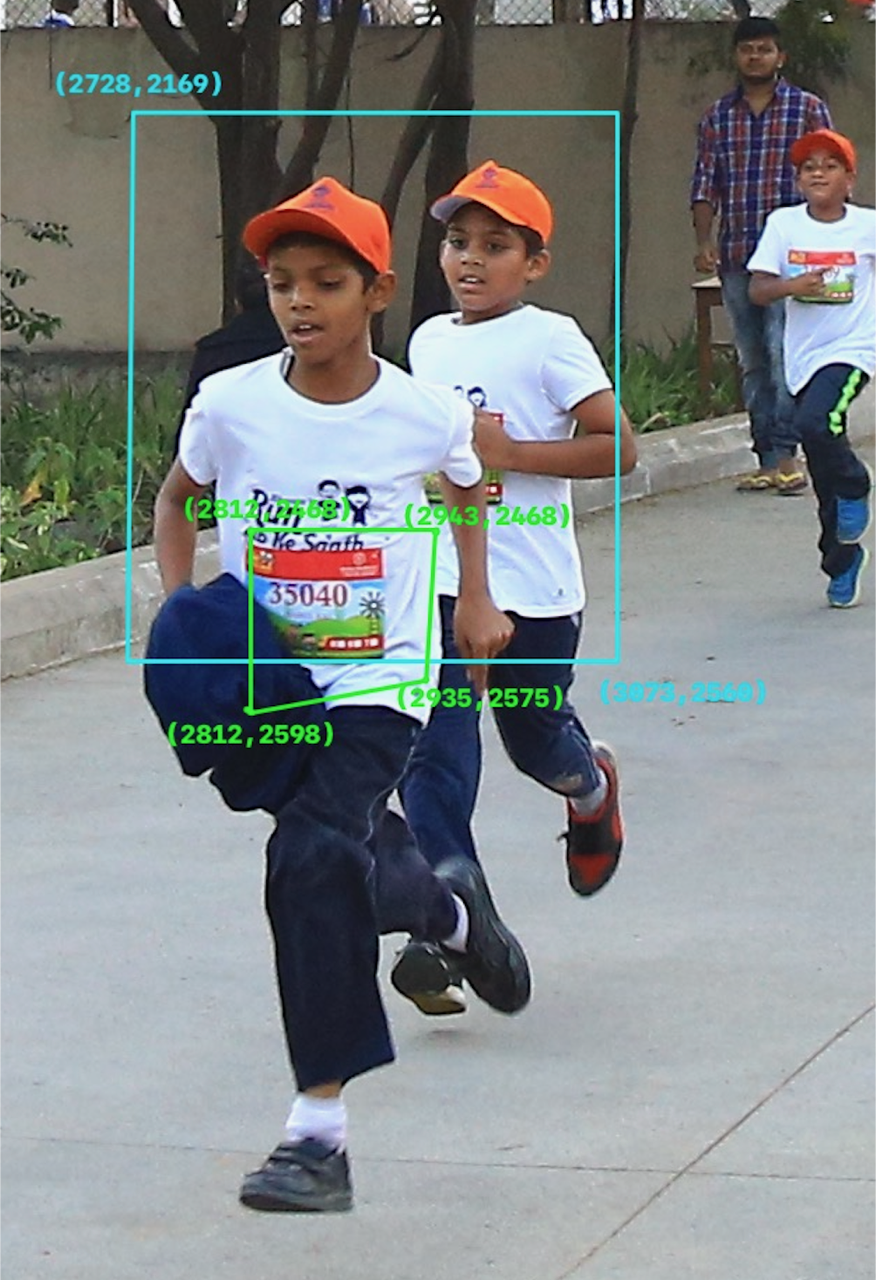
\includegraphics[width=\textwidth]{images/dataset/BadTagging_Overlap}
  \end{subfigure}
  \hspace{\fill}
  \begin{subfigure}[b]{0.3\textwidth}
    
\includegraphics[width=\textwidth]{images/dataset/BadTagging_NotAroundFace}
  \end{subfigure}
  \hspace{\fill}  
  \begin{subfigure}[b]{0.2\textwidth}
    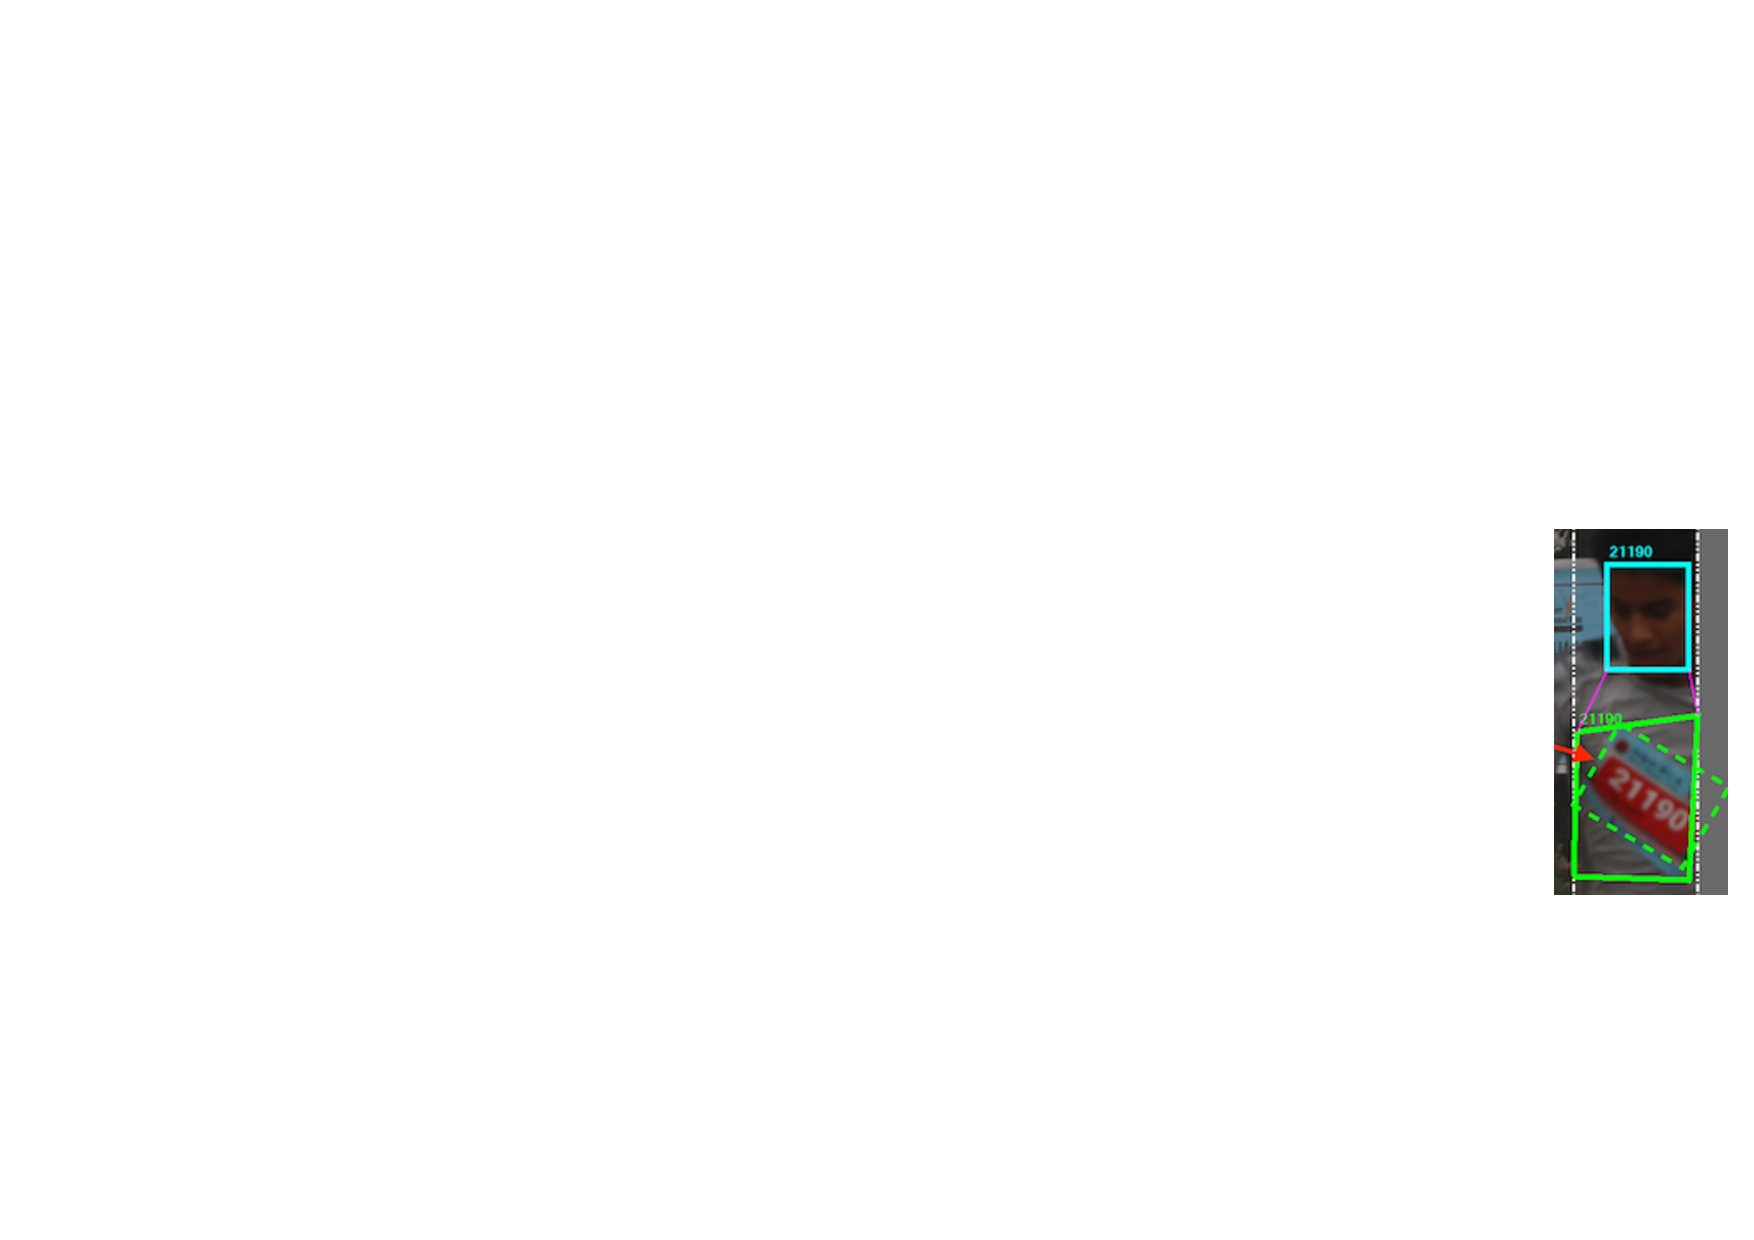
\includegraphics[width=\textwidth]{images/dataset/BadTagging_NotAroundBib}
  \end{subfigure}
  \hspace{\fill}
  
  \caption[Product testing issues identified]{Issues identified from rounds of external testing to the tagging team. Cyan lines indicate face regions, lime lines indicate bib regions, magenta lines indicate bib-to-face guidelines. \textit{Clockwise:} Face region is too far away from bib region; bib region is poorly marked (dotted lines expected); face region is too small (dotted lines expected); face region overlaps bib region.}
  \label{fig:dataset:issues_with_tagging}
\end{figure}
